\section{The TGCT Framework}
TGCT is a framework for crowdsourced testing of Android application. As shown in Figure\ref{fig:arch}, TGCT works in the following process: (1) Corresponding to different events, TGCT builds the GUI model, which describes the transition between different windows. (2) According to the test tasks which composed of uncommon window transitions(test cases) and uncovered window transitions, TGCT predicts the test preference of crowd workers through collaborative filtering algorithm. (3) Starting from the workers' current window, TGCT calculates the path to the target test task, by which the workers complete the path transition to reproduces the exceptions or triggers new exceptions.
\begin{figure}[htbp]
\centering
\centerline{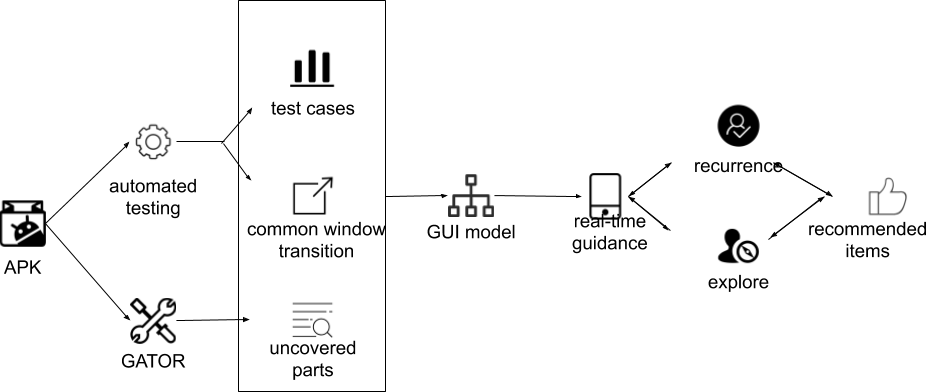
\includegraphics[width=\columnwidth,height=4cm]{fig/2.png}}
\caption{The process of TGCT.}
\label{fig:arch}
\end{figure}

\subsection{Representation of GUI Model}
GUI model is build in a directed graph structure: 
\begin{equation}
G = < W, E >
\end{equation}
where W represents the window set, and E represents the event set. Window refers to the Activity, Dialog, and Menu in the Android application. TGCT describes events by three attributes. The event $e_{i}$ converts to a vector:
\begin{equation}
e_{i} = \{w\_s_{i}, w\_t_{i}, m_{i}, t_{i}, c_{i}\}
\end{equation}

In the event i, $w\_s_{i}$ represents the starting window, the $w\_t_{i}$ represents the target window, and $m_{i}$ represents the screenshots in the test process. $t_{i}$ records the timestamp when the event occurred, and the $c_{i}$ is set to distinguish the window transition type in GUI model. The three types are common window transition, uncommon window transition(test cases) and the uncovered window transition.

Taking the starting window as the starting node, the target window as the termination node, TGCT traverse the sequence of test events and connect a directed edge between starting node and termination node. Finally, these directed edges form a directed graph.

% TGCT defines some fields of the edge to represent the window transition set triggered by the event. , "event\_type" records event type, "event\_handlers" corresponds to "message" in automated test events, "image\_URL" represents the screenshots in the test process, and "message" field represents exception message that test event triggers, "create\_time" save the timestamp when the event occurred. TGCT sets the "data\_type" field to distinguish the window transition type in GUI model. Among them, 1 represents the common window transition, 2 represents the uncommon window transition(test cases) triggering the exception, and 0 represents the uncovered window transition.


\subsection{Construction of GUI Model}
%Figure\ref{fig:flow_chart} shows the process of GUI model construction. 
Requesters upload Android application APK on the crowdsourced platform. TGCT parses APK by automated testing and static source code anlysis respectively, and generates a GUI model. The model includes three parts:
(1) common window transitions that do not trigger exceptions, (2) uncommon window transitions(test cases) that trigger exceptions, (3) uncovered window transition supplemented by static analysis.
%\begin{figure}[htbp]
%\centering
%\centerline{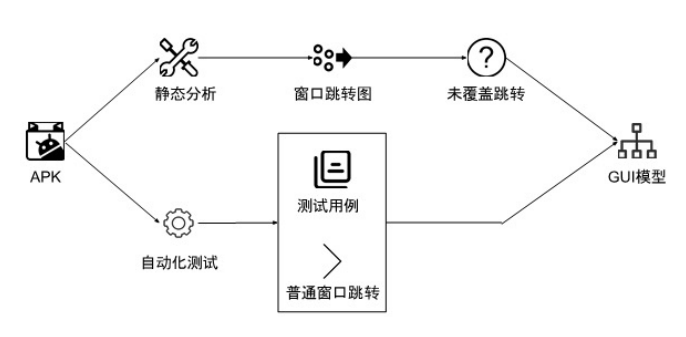
\includegraphics[width=\columnwidth,height=4cm]{fig/3.png}}
%\caption{The process of GUI model construction.}
%\label{fig:flow_chart}
%\end{figure}

%common window transition%
\subsubsection{Common Window Transition}
Directed by automated test, TGCT traverses all components in Android, then generates a sequence of test events, and saves a screenshot when the test event occurs. Based on the section 2.1, TGCT represents the test event as the edge.
% Some fields must be recorded by test events. The "time" field represents the time when the event occurred, and the "activityBeforeAction" field and the "activityAfterAction" field record the windows before and after the event, respectively. The "type" field represents the event type, and the "message" field represents event information in detail.


% TGCT defines some fields of the edge to represent the window transition set triggered by the event. "source\_node" and "target\_node" store the names of starting window and target window, "event\_type" records event type, "event\_handlers" corresponds to "message" in automated test events, "image\_URL" represents the screenshots in the test process, and "message" field represents exception message that test event triggers, "create\_time" save the timestamp when the event occurred. TGCT sets the "data\_type" field to distinguish the window transition type in GUI model. Among them, 1 represents the common window transition, 2 represents the uncommon window transition(test cases) triggering the exception, and 0 represents the uncovered window transition.

During the implement, TGCT uses the automated testing framework of MoocTest platform\footnote{www.mooctest.net} to generate test events in the format of Json, and builds GUI Model to realize flexible Json parsing, according to Json data structure. 

% TGCT chooses the automated testing framework of MoocTest platform\footnote{www.mooctest.net}. This framework traverses all components in Android by depth-first algorithm, then generates a sequence of test events, and saves a screenshot when the test event occurs. The automated testing framework records the sequence of events in the format of Figure\ref{fig:foramt}. The "time" field represents the time when the event occurred, and the "activityBeforeAction" field and the "activityAfterAction" field record the windows before and after the event, respectively. The "type" field represents the event type, and the "message" field represents event information in detail.
% \begin{figure}[htbp]
% \centering
% \centerline{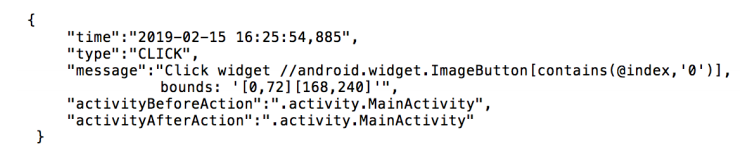
\includegraphics[width=\columnwidth,height=2cm]{fig/4.png}}
% \caption{The format of event sequence.}
% \label{fig:foramt}
% \end{figure}


%By traversing the sequence of test events, TGCT take the window before the event triggered as the starting node("activityBeforeAction"), the window after the event triggered as the termination node("activityAfterAction"), connect a directed edge. Finally these edges form a directed graph.
%Traversing event sequences, TGCT stores GUI state changes recorded by automated tests in a directed graph structure: G = < N, E >, where N represents the set of points, which represents the set of Android application layer windows, and E represents the edge set, which represents the window transition set triggered by the event.


% The automated test framework saves a screenshot of the current running state of the application,and names it with the current timestamp. The TGCT mechanism combines the coordinates of event-related components to mark the window components, assists in describing events, and provides clear test guidance. The processing of the screenshot information are as follows: (1) \textbf{Correspond screenshots to events:} Read the screenshots list P. For any screenshots $p_{i}$, whose file name is $n_{i}$, an edge $e_{i}$ can be found in the application edge set E. It satisfies the corresponding timestamp $t_{i}$, which is greater than $n_{i}$ and closest to $n_{i}$. The mapping relationship between $p_{i}$ and $e_{i}$ is established.
% (2) \textbf{Associate user interaction events and corresponding screenshots:} an Android application contains multiple components, so how does TGCT describe the test event-related components to crowdsourced workers? On the one hand, for the user interaction test event, the TGCT draws the component in the screenshot according to the component coordinates recorded in the corresponding test event, then TGCT feeds it back to the worker. On the other hand, for the system test event, the TGCT does not modify the original screenshot, but just saves it.

\subsubsection{Uncommon Window Transition}
The TGCT collects application runtime exceptions by automated testing, and generates the sequence of exception log. Traversing the sequence of exception log, TGCT analyzes each log and find the corresponding edge according to timestamp(one edge corresponds to one window transition). By changing the edge of the GUI model with the attribute $c_{i}$ to indicate that the corresponding edge belongs to the uncommon window transition. With this, TGCT takes the uncommon window transition as the test case.

% The format of each log is as shown in Figure\ref{fig:foramt2}.

% and modify the "data\_type" field of the edge to 2 and save the "LOG" information to "message" field of the edge. With this, TGCT takes the uncommon window transition as the test case.

%The automated testing framework exports program run logs, each of which is formatted as shown in Figure\ref{fig:foramt2}. When the application starts, the Android system opens a new thread of execution for it, which generates other sub-threads and runs other windows of the application in the sub-threads. Threads are distinguished by thread ID as a unique identifier. In program log, thread ID is used as identifier to record resource loading process and program running status in different threads. The "type" field records the debugging information of the program log, the "LOG" field receives the information from the program's specific code, and the "time" field stores the timestamp generated by the exception. 
% \begin{figure}[htbp]
% \centering
% \centerline{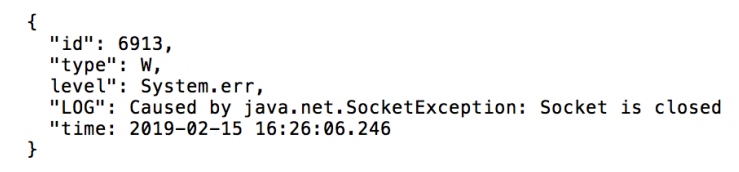
\includegraphics[width=\columnwidth,height=2cm]{fig/5.png}}
% \caption{The format of program log.}
% \label{fig:foramt2}
% \end{figure}

%For any log $l_{i}$ in the exception log set L, its corresponding time is $t_{i}$. In the edge set E, there must be an edge $e_{i}$, whose occurrence time is less than $t_{i}$ and closest to $t_{i}$. The TGCT mechanism searches for the corresponding event information for each exception log, modifies the window transition information, sets the "data\_type" field to 2, and outputs the "LOG" information in the log to the "message" field.

\subsubsection{Uncovered Window Transition}
Based on the static analysis method of Android source codes, the directed graph $G_{1}$ was proposed to detect the callback in programs. The callback information of window transition is recorded in the edge of the $G_{1}$. A new attribute is designed to store the window name where the callback function occurs and the definition of the callback function. $G_{1}$ establishes the mapping between callback function and GUI model.

% The "source\_node" field and the "target\_node" field store the name of the starting node and the target node. The "event\_handlers" field stores the window name where the callback function occurs and the definition of the callback function. $G_{1}$ establishes the mapping between callback function and GUI model.

The TGCT traverses the edges of $G_{1}$, retrieves the event information of automated testing, and determines whether the window transition has been covered by automated testing. If the window transition is not included, the TGCT stores the edge information from $G_{1}$ in the format of uncovered window transition. 

Based on the work of Yang, Shengqiang et al.\cite{b5} developed a tool GATOR, which generates window transition graph (WTG). With the GATOR tool, TGCT constructs a directed graph WTG to record callback information, which is a worthy addition to the test cases detected by automated testing framework.

% The callback information of window transition is recorded in the edge of the graph, and the information contained in each edge is shown in Figure\ref{fig:info}. The "source\_node" field and the "target\_node" field store the name of the starting node and the target node. The "event\_handlers" field stores the window name where the callback function occurs and the definition of the callback function. GATOR establishes the mapping between callback function and GUI model. %By analyzing the name and definition of callback function, the event information corresponding to callback function is stored in the "type" field.
% \begin{figure}[htbp]
% \centering
% \centerline{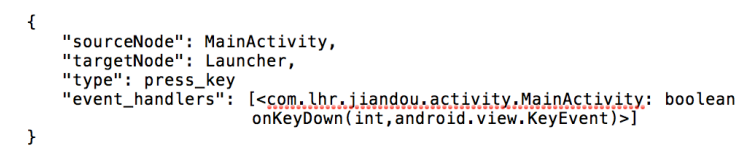
\includegraphics[width=\columnwidth,height=2cm]{fig/6.png}}
% \caption{The information of edge in WTG.}
% \label{fig:info}
% \end{figure}

\subsection{Test Task recommendation Module}
The TGCT uses an item-based collaborative filtering algorithm to implement a test task recommendation module for test cases and uncovered windows. Cold start is a problem that must be faced in the collaborative filtering algorithm. Combining with GUI model in section 2.1, TGCT analyses the attributes of different window transitions to solves the cold start problem. Figure\ref{fig:recomd} shows the process of the recommendation module. 
\begin{figure}[htbp]
\centering
\centerline{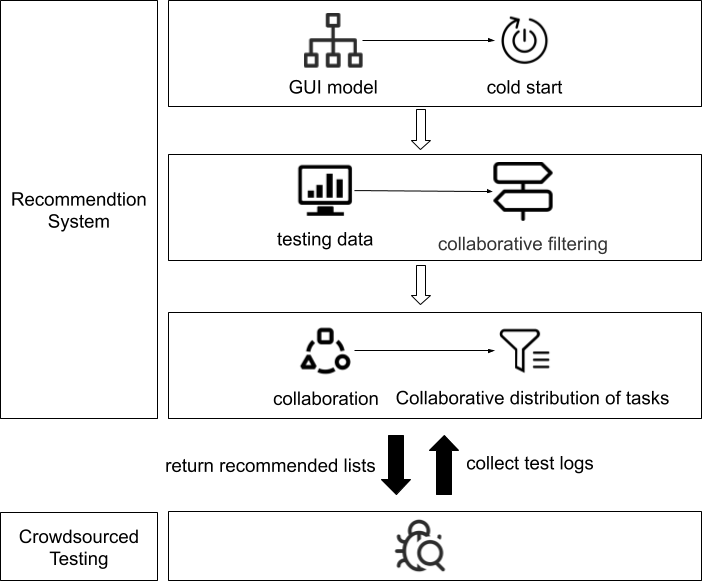
\includegraphics[width=7cm,height=6cm]{fig/7.png}}
\caption{The process of the recommendation module.}
\label{fig:recomd}
\end{figure}
\subsubsection{Cold Start}
In recommendation module for uncovered window transition, because uncovered window transition is difficult to find out the representative exception attributes, the TGCT mechanism adopts random strategy to solve the cold start problem. 

%This paper mainly solve the cold-start problem of recommendation module for uncommon window transitions from two aspects: cold-start for users and cold-start for items. The steps are as follows:(1)\textbf{Classification of exceptions:} Collect and understand the exception information in GUI model. TGCT mechanism classifies common exceptions in Android applications and manually evaluates the severity of exceptions. The higher the score, the more serious it is.(2)\textbf{Exception selection:} According to the exception distribution of the current application, the TGCT mechanism randomly selects exceptions from each type to form test cases and recommend them to each new crowd worker.

%So far, TGCT elaborates the solution of cold start problem for users. Based on this, 
In recommendation module for test cases, TGCT classifies exceptions in Android applications, and randomly select exceptions from each category evenly to recommend to new crowd workers. Besides, the TGCT studies the solution of cold start for new test cases. TGCT calculates the similarity between different test cases based on the cosine similarity by analyzing the properties of the anomaly, and realizes the coarse-grained personalized recommendation.

Based on the GUI model constructed in 2.1, TGCT describes test cases by three attributes. The test case $t_{i}$ converts to a vector:
\begin{equation}
t_{i} = {(e_{1}, w_{1}),(e_{2}, w_{2}),(e_{3}, w_{3})}
\end{equation}

$e_{1}$ represents the exception type, and the weight $w_{1}$ depends on the severity of the exception defined manually. $e_{2}$ represents the starting window of an exception, and $w_{2}$ represents the page level of the window. For any window $w_{i}$, the corresponding page level $l_{i}$ is equal to the shortest path from MainActivity to $w_{i}$ plus 1.
%From the point of view of improving test coverage, the deeper the nesting of windows, the more difficult it is to detect abnormalities, and the higher the weight it gives, the more it is recommended to crowd workers.
$e_{3}$ represents the event type, and the TGCT mechanism assigns different weights to different event types.

Test cases are represented by vectors, and the similarity $S_{AB}$ between test case A and test case B is calculated by cosine similarity in TGCT mechanism, where $A_{i}$ represents an attribute value in the vector of test case A:
\begin{equation}
S_{AB} = \frac{AB}{||A||||B||} = \frac{\sum_{i = 1}^nA_i \times B_i}{\sqrt{\sum_{i = 1}^nA_i^{2}} \times \sqrt{\sum_{i = 1}^nB_i^{2}}}
\end{equation}

\subsubsection{Item-Based Collaborative Filtering Recommendation}
The first five minutes of crowdsourced testing is the cold start stage of the recommendation module. After collecting preference data of crowd worker, the recommendation module is completed by using the collaborative filtering algorithm based on items. Given the test cases selected by the current crowd worker u, the preferences for other unselected test cases are calculated. The calculation steps are as follows: (1) Compute the similarity between test cases: TGCT records the selection of different test cases by crowd workers. Based on the data, the similarity between different test cases is calculated. Similarity $w_{ij}$ between test case i and test case j are calculated using the following formula:
\begin{equation}
w_{ij} = \frac{|N(i) \cap N(j)|}{\sqrt{|N(i) \cup N(j)|}}
\end{equation}
N(i) denotes the group of workers who choose test case i to test, and N(j) denotes the group of workers who choose test case j to test.
%N(i) denotes the group of workers who choose test case i to test, and N(j) denotes the group of workers who choose test case j to test. $N(i) \cap N(j)$ represents the crowd worker set that chooses both test case i and test case j. Among the crowd workers who choose test case i, the more workers choose test case j, the higher the similarity between test case i and test case j is.

(2) Predict the preference of crowd workers for other test cases: According to the historical test cases named N(u) chosen by crowd workers u, the preference degree $p_{uj}$ of crowd workers u to test case j is predicted by TGCT based on KNN. The calculation formula is as follows:
\begin{equation}
p_{uj} = \sum_{i\in N(u) \cap S(j,k)}w_{ij}r_{ui}
\end{equation}
S(j,k) represents the set of k test cases closest to test case j. $r_(ui)$ represents the preference degree of crowd workers u for test case i. 
%S(j,k) represents the set of k test cases closest to test case j. In the test case set N(u) which has been tested by crowd workers u, for each test case i, the similarity $w_(ji)$ between test case j and test case i is calculated. $r_(ui)$ represents the preference degree of crowd workers u for test case i. In the mechanism of TGCT, the value of $r_(ui)$ is between {0,1}. If crowd worker u chooses test case i, $r_(ui)$ = 1, otherwise, it is 0. 

(3) Generate test lists in Top-N mode: N test cases with the highest preference are selected and returned to the current crowd worker.%The recommended module for uncovered window transitions is the same above.

\subsubsection{Collaborative Test Task Assignment}
%In Android crowdsourced test with N participants, 
TGCT defines the concept of "verified exception" for test cases T = {$t_{1}$, $t_{2}$,...}. In the crowdsourced testing process, if the test case $t_{i}$ is tested more than the threshold S times, its corresponding exceptions are considered to have been verified and will not appear in the recommended list. Recommendation module will guide crowd workers to verify and explore other exceptions.%, optimize crowdsourced resource allocation, and improve the test coverage and efficiency.

\subsection{Real-time Guide Mechanism}
%The TGCT is integrated into the mobile phone with Android SDK. 
Figure\ref{fig:guide} shows how the TGCT mechanism guides crowd workers to complete their testing tasks on the Android.
%The TGCT judges the type of test task chosen by crowd workers. If it is a test case, it guides crowd workers to repeat abnormalities. If it is a transition from uncovered windows, it guides crowd workers to reach the starting window and explore new abnormalities.
\begin{figure}[htbp]
\centering
\centerline{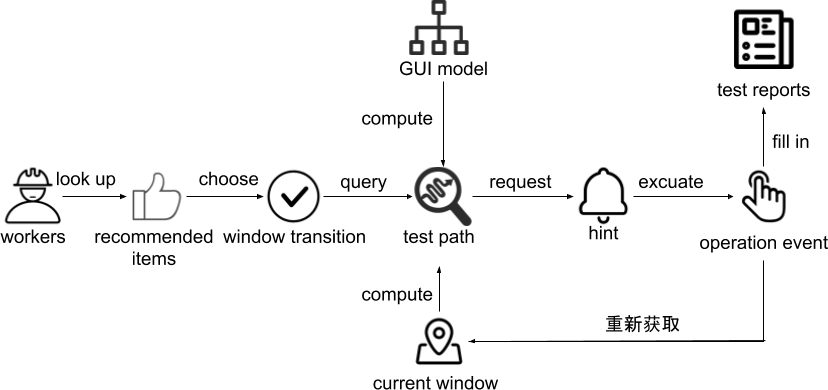
\includegraphics[width=\columnwidth,height=4.5cm]{fig/10.png}}
\caption{The process of the guide mechanism.}
\label{fig:guide}
\end{figure}

%Real-time guide consists of two steps. Firstly, TGCT calculate the transition path. Secondly, TGCT 
%First, the crowdsourced worker is guided to reach the starting window of the target window transition from the current window. Secondly, for the test case, the TGCT guides the crowdsourced worker to execute the operation event that triggers the exceptions in the starting window, and for the uncovered window transition ,TGCT mechanism prompts the crowdsourced worker to complete the window transition event.The following will introduce the real-time boot design of the Android application from the transition path calculation and the real-time prompt.

\subsubsection{Transition Path}
We define the prep-event sequence as the sequence of events before one event. TGCT calculates the transition path based on the prep-event to reproduce the exceptions triggered by the test case. By fixing target window transition t selected by the crowd worker, TGCT defines the starting window corresponding to t as $w_{s}$, and the current window for the crowd worker as $w_{c}$.
There are three steps as follows:
(1) \textbf{Find the lowest common ancestor(LCA) $w_{father}$ of $w_{c}$ and $w_{s}$ in GUI model:} The LCA of $w_{c}$ and $w_{s}$ in GUI is the shared ancestor of $w_{c}$ and $w_{s}$ that is located farthest from the root.
(2) \textbf{Find the prep-event sequence from $w_{s}$ to $w_{father}$:} Let the target window transition t as the current window transition, and the event corresponding to t as the current event. TGCT can lookup the window transition set with $w_{s}$ as the target window. Searching for the set, TGCT selects one window transition as the prep-event, which satisfies the corresponding timestamp is smaller than the time of current event and closest to it. Let the prep-event as the current event, TGCT repeats the same operation above until the starting window of the prep-event sequence is $w_{father}$.
(3) \textbf{Find the shortest path from $w_{c}$ to $w_{father}$:} TGCT considers that the path from $w_{c}$ to $w_{father}$ is common event sequence. TGCT only needs to calculate the shortest transition path through breadth-first traversal.

% There are three steps of calculating the shortest transition path:
% (1) Remove the program's promotion window because these promotion windows only face to the new user and they are not meaningful. Start test from the MainActivity.
% (2) Construct an undirected graph based on the GUI model of step 1.
% (3) Calculate the shortest path through breadth-first traversal.
For crowd workers who choose the uncovered window transition, TGCT calculates the shortest path from $w_{c}$ to $w_{s}$ based on step (3).

\subsubsection{Real-time Guidance}
According to the location information of crowd workers, the mechanism of TGCT chooses window transition according to different rules to realize real-time prompting and guidance. 
%The status of crowd workers in the test path can be divided into the following categories:1. The starting window but not the starting window of target window transition(edge).2. The starting window of target window transition(edge) but reached the first time.3. The end window of target window transition(edge).